\documentclass[letterpaper]{article}
\usepackage[submission]{aaai2027}
\usepackage[hyphens]{url}
\usepackage{graphicx}
\usepackage{amsmath,amssymb,amsthm}
\usepackage{booktabs}
\usepackage{algorithm}
\usepackage{algorithmic}
\usepackage{tikz}
\usepackage{pgfplots}
\pgfplotsset{compat=1.18}
\usepgfplotslibrary{groupplots}
\urlstyle{rm}
\def\UrlFont{\rm}
\frenchspacing
\setlength{\pdfpagewidth}{8.5in}
\setlength{\pdfpageheight}{11in}
\pdfinfo{
/TemplateVersion (2027.1)
}

\setcounter{secnumdepth}{0}
\newtheorem{theorem}{Theorem}
\newtheorem{corollary}{Corollary}
\newtheorem{proposition}{Proposition}
\definecolor{accsblue}{RGB}{15,77,146}
\definecolor{coptred}{RGB}{182,67,66}
\definecolor{crcgreen}{RGB}{66,148,158}
\definecolor{globalgray}{RGB}{150,150,150}
\definecolor{targetgray}{RGB}{110,110,110}

\pgfplotsset{
  paperaxis/.style={
    tick label style={font=\small},
    label style={font=\small},
    title style={font=\normalsize, align=left},
    legend style={font=\small, draw=none, fill=none},
    axis line style={black, line width=0.7pt},
    tick style={black, line width=0.6pt},
    major grid style={draw=none},
    every axis plot/.append style={line width=0.9pt},
  }
}

\newcommand{\FigureSelectionAmplificationTikZ}{%
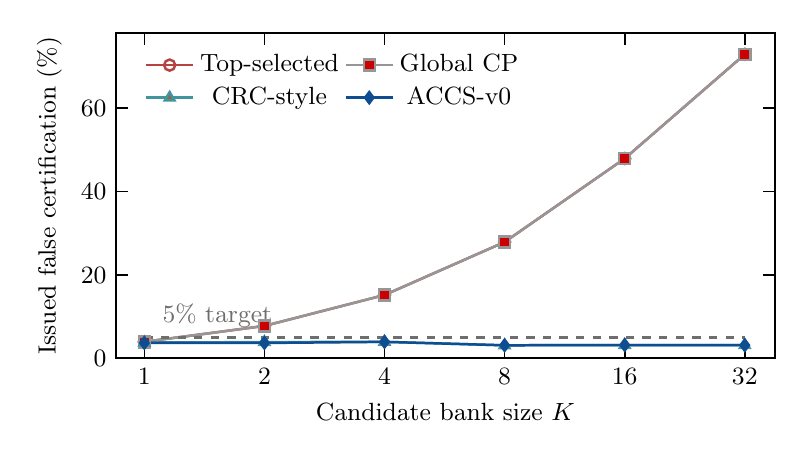
\begin{tikzpicture}
\begin{axis}[
  paperaxis,
  width=0.82\textwidth,
  height=2.25in,
  xmode=log,
  log basis x=2,
  xmin=0.85,
  xmax=38,
  ymin=0,
  ymax=78,
  xtick={1,2,4,8,16,32},
  xticklabels={1,2,4,8,16,32},
  ytick={0,20,40,60},
  xlabel={Candidate bank size $K$},
  ylabel={Issued false certification (\%)},
  legend columns=2,
  legend pos=north west,
]
\addplot+[mark=o, color=coptred] coordinates {
  (1,3.99) (2,7.79) (4,15.20) (8,27.90) (16,47.91) (32,72.88)
};
\addlegendentry{Top-selected}
\addplot+[mark=square*, color=globalgray] coordinates {
  (1,3.99) (2,7.79) (4,15.20) (8,27.90) (16,47.91) (32,72.88)
};
\addlegendentry{Global CP}
\addplot+[mark=triangle*, color=crcgreen] coordinates {
  (1,3.81) (2,3.92) (4,3.98) (8,3.15) (16,3.22) (32,3.17)
};
\addlegendentry{CRC-style}
\addplot+[mark=diamond*, color=accsblue] coordinates {
  (1,3.72) (2,3.71) (4,3.98) (8,3.15) (16,3.22) (32,3.17)
};
\addlegendentry{ACCS-v0}
\addplot[dashed, color=targetgray] coordinates {(1,5) (32,5)};
\node[anchor=south west, font=\small, text=targetgray] at (axis cs:1.05,5) {5\% target};
\end{axis}
\end{tikzpicture}%
}

\newcommand{\FigureAuditLayersTikZ}{%
\begin{minipage}[t]{0.48\textwidth}
\centering
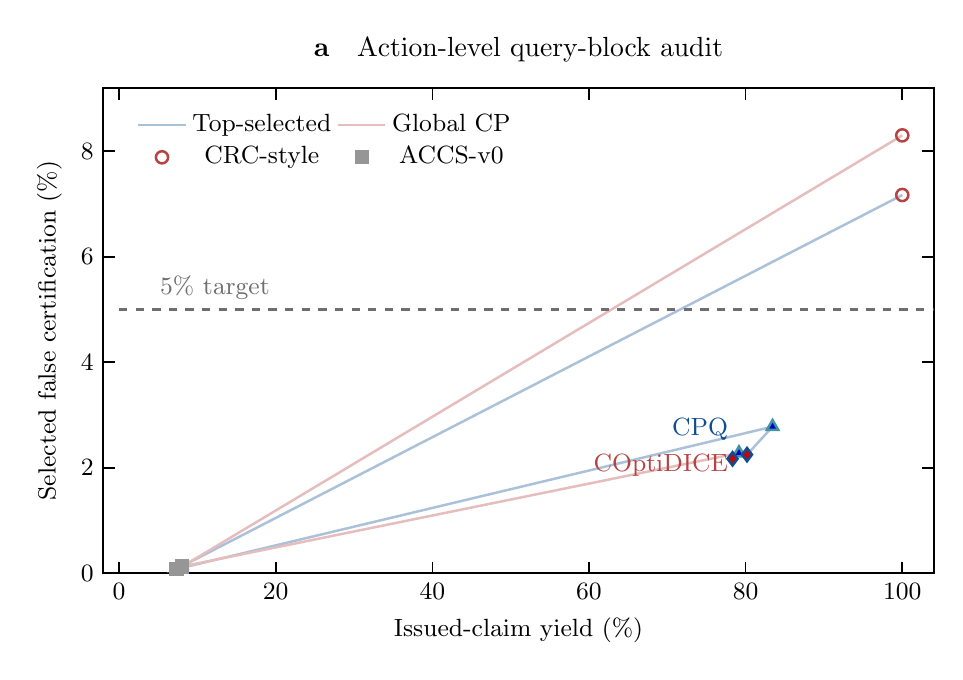
\begin{tikzpicture}
\begin{axis}[
  paperaxis,
  width=\linewidth,
  height=3.05in,
  xmin=-2,
  xmax=104,
  ymin=0,
  ymax=9.2,
  xtick={0,20,40,60,80,100},
  ytick={0,2,4,6,8},
  xlabel={Issued-claim yield (\%)},
  ylabel={Selected false certification (\%)},
  title={\textbf{a}\quad Action-level query-block audit},
  legend columns=2,
  legend pos=north west,
]
\addplot[color=accsblue!35] coordinates {(100,7.17) (7.33,0.08) (83.44,2.78) (80.18,2.25)};
\addplot[color=coptred!35] coordinates {(100,8.30) (8.08,0.13) (79.15,2.28) (78.33,2.17)};
\addplot+[only marks, mark=o, mark size=2.2pt, color=coptred] coordinates {(100,7.17) (100,8.30)};
\addlegendentry{Top-selected}
\addplot+[only marks, mark=square*, mark size=2.1pt, color=globalgray] coordinates {(7.33,0.08) (8.08,0.13)};
\addlegendentry{Global CP}
\addplot+[only marks, mark=triangle*, mark size=2.4pt, color=crcgreen] coordinates {(83.44,2.78) (79.15,2.28)};
\addlegendentry{CRC-style}
\addplot+[only marks, mark=diamond*, mark size=2.4pt, color=accsblue] coordinates {(80.18,2.25) (78.33,2.17)};
\addlegendentry{ACCS-v0}
\addplot[dashed, color=targetgray] coordinates {(0,5) (104,5)};
\node[anchor=south west, font=\small, text=targetgray] at (axis cs:4,5) {5\% target};
\node[anchor=east, font=\small, text=accsblue] at (axis cs:79.0,2.72) {CPQ};
\node[anchor=east, font=\small, text=coptred] at (axis cs:79.0,2.05) {COptiDICE};
\end{axis}
\end{tikzpicture}
\end{minipage}\hfill
\begin{minipage}[t]{0.48\textwidth}
\centering
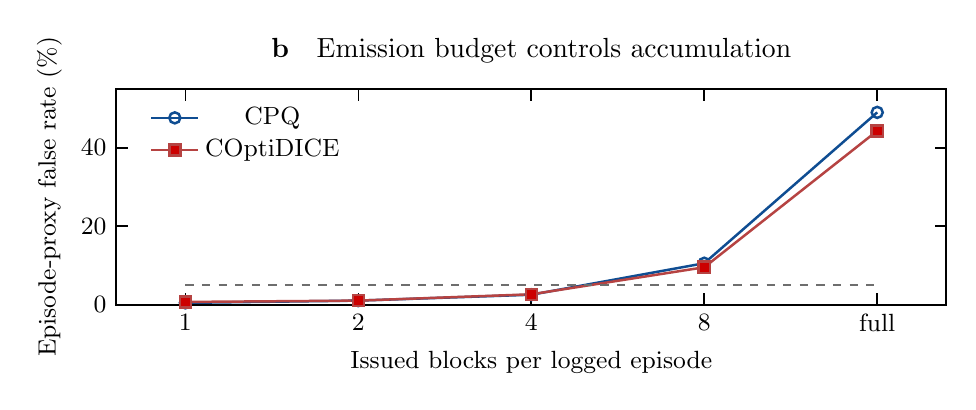
\begin{tikzpicture}
\begin{axis}[
  paperaxis,
  width=\linewidth,
  height=1.7in,
  ymin=0,
  ymax=55,
  symbolic x coords={1,2,4,8,full},
  xtick=data,
  xlabel={Issued blocks per logged episode},
  ylabel={Episode-proxy false rate (\%)},
  title={\textbf{b}\quad Emission budget controls accumulation},
  legend pos=north west,
]
\addplot+[mark=o, color=accsblue] coordinates {(1,0.46) (2,1.03) (4,2.53) (8,10.57) (full,49.08)};
\addlegendentry{CPQ}
\addplot+[mark=square*, color=coptred] coordinates {(1,0.69) (2,1.03) (4,2.64) (8,9.54) (full,44.37)};
\addlegendentry{COptiDICE}
\addplot[dashed, color=targetgray] coordinates {(1,5) (full,5)};
\end{axis}
\end{tikzpicture}

\vspace{0.18in}
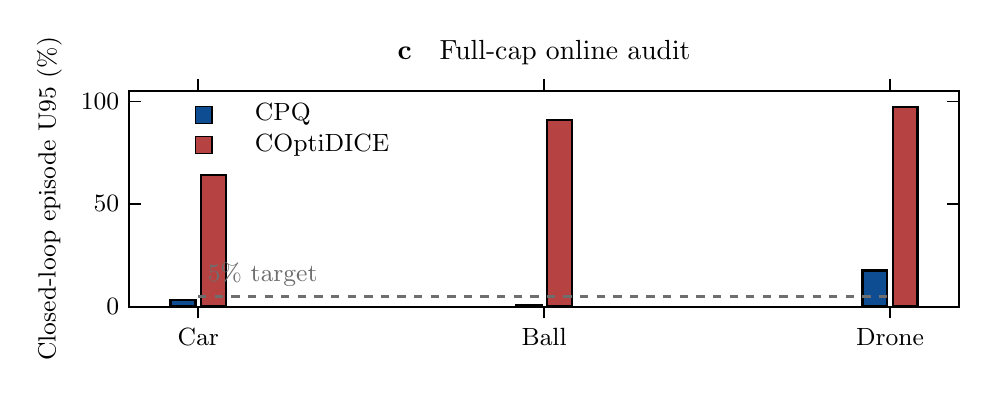
\begin{tikzpicture}
\begin{axis}[
  paperaxis,
  width=\linewidth,
  height=1.7in,
  ybar,
  bar width=9pt,
  ymin=0,
  ymax=105,
  symbolic x coords={Car,Ball,Drone},
  xtick=data,
  ylabel={Closed-loop episode U95 (\%)},
  title={\textbf{c}\quad Full-cap online audit},
]
\addplot+[fill=accsblue, draw=black] coordinates {(Car,3.22) (Ball,0.50) (Drone,17.61)};
\addplot+[fill=coptred, draw=black] coordinates {(Car,64.15) (Ball,90.89) (Drone,97.23)};
\addplot[dashed, color=targetgray, sharp plot] coordinates {(Car,5) (Drone,5)};
\node[anchor=south west, font=\small, text=targetgray] at (axis cs:Car,5) {5\% target};
\node[draw=black, fill=accsblue, minimum width=6pt, minimum height=6pt, inner sep=0pt] at (rel axis cs:0.09,0.89) {};
\node[anchor=west, font=\small] at (rel axis cs:0.14,0.89) {CPQ};
\node[draw=black, fill=coptred, minimum width=6pt, minimum height=6pt, inner sep=0pt] at (rel axis cs:0.09,0.75) {};
\node[anchor=west, font=\small] at (rel axis cs:0.14,0.75) {COptiDICE};
\end{axis}
\end{tikzpicture}
\end{minipage}%
}


\title{A Safety Score Is Not a Certificate: Calibration After Action Selection in Offline RL}

\author{
    Anonymous Submission
}
\affiliations{
    Paper ID withheld for double-blind review.
}

\begin{document}

\maketitle

\begin{abstract}
A learned safety score is not a deployment certificate. Offline safe
reinforcement learning systems increasingly attach safety scores or
residual-budget claims to actions selected from learned candidate banks. We
study false safety claims among the actions actually issued after deployment
selection, a target distinct from policy training, marginal calibration, or
average constraint satisfaction. Candidate generation, reward ranking, support
filtering, and fallback logic can concentrate rare calibration failures on the
selected action. We formalize selective safety certification over fixed query
blocks, give finite-family audit guarantees for issued-claim risk and
episode-budgeted claims, and instantiate the protocol as support-aware ACCS.
On trained CAPSIQL, CPQ, and COptiDICE proposers on official DSRL CarCircle,
top-action false certification reaches 7.17\% and 8.30\% in the high-signal
CPQ/COptiDICE rows, while ACCS-v0 reduces issued false certification to
2.25\%/2.17\% with 80.18\%/78.33\% yield. A pre-registered fixed-cap
closed-loop frontier separates proposer-environment pairs: CPQ certifies full
CarCircle and BallCircle episodes with exact 95\% episode-risk upper bounds of
3.22\% and 0.50\%, whereas COptiDICE reaches 64.15\% and 90.89\%. These
results make post-selection auditing a certificate evidence layer: it can
certify particular issued-claim contracts and reject unsafe or unsupported
contracts, but it is not a replacement for safe policy learning.
\end{abstract}

\section{Introduction}

Offline safe reinforcement learning is increasingly used as a decision layer
for systems that must trade reward against state-dependent safety budgets.
Modern methods learn cost-aware critics, budget-conditioned policies, and
constraint-adaptive action filters for offline safe RL~\cite{li2025caps,wang2026bcrl}.
Other recent directions build almost-sure safety or flow-policy
formulations~\cite{aegis2026,tayal2026safefql}. These components are useful for
choosing actions, but they do not by themselves answer a different statistical
question: when the deployed system issues a safety claim for its selected
action, how often is that claim false?

The distinction matters because deployment systems do not certify random
candidate actions. They generate a bank of candidates, filter by a requested
residual budget, rank by reward, apply fallback rules, and often repeat this
process under changing constraints. Marginal calibration over candidate
proposals can therefore leave the selected action miscalibrated. In a simple
construction, each proposed action has only 4\% false-certification probability,
but selecting the best of 16 reward-ranked candidates raises the issued-claim
false-certification rate to about 48\%. Calibration before action selection is
not calibration after action selection.

This paper studies the missing evidence object: false certification among
issued action claims. We define a deployment query block containing the state,
residual budget, candidate action bank, learned reward and safety scores,
support evidence, and residual-cost labels under a declared continuation
policy. This target is related to selective conformal and conformal risk-control
ideas~\cite{bao2025cap,angelopoulos2025crc}, but the RL setting adds candidate
selection, support, and continuation-policy dependence. A certification rule
either issues one action certificate or abstains.
The target risk is the ratio of expected false issued claims to expected issued
claims, and it must be reported together with yield to avoid vacuous safety by
abstention.

This formulation changes what a valid evaluation must hold fixed. If an auditor
is tested on easier candidates than the deployed proposer emits, low risk says
little about deployment. If residual costs are labeled under one continuation
policy but deployed under another, the certificate target has changed. If a
rule issues on actions outside logged support, no distribution-free offline
calibration can identify the missing residual outcomes. We therefore treat the
query law, residual-label protocol, and support evidence as part of the
certification problem rather than implementation details.

Our method is a support-aware selective auditor over fixed query blocks. The
auditor compares a prespecified family of certification rules using independent
audit blocks, selects rules whose upper confidence bound on issued-claim risk
is below the target, and breaks ties by utility or yield. This design treats
support as evidence rather than decoration: unsupported actions, policy-mismatched
residual labels, and low-yield global thresholds are all diagnosed rather than
silently certified.

The main line is that a certificate must be audited after action selection
under a frozen deployment contract. Around that line, we make three
contributions. First, we isolate selected safety certification as an estimand
for offline safe RL and prove that marginal candidate calibration can fail
after reward-based action selection. Second, we give a finite-family audit
protocol that controls issued-claim risk with explicit yield, support, and
residual-policy accounting. Third, we build an empirical evidence stack from
action-level query blocks to logged episode proxies and true closed-loop
fixed-cap audits, making clear where action certificates do and do not imply
trajectory-level claims.

The empirical result is already visible on trained safe-RL proposers, not only
on exact toys. On official DSRL CarCircle, we audit CAPSIQL, CPQ, and COptiDICE
checkpoint proposers under the same query-bank and residual-label
contract~\cite{liu2023dsrl,li2025caps}. Global candidate conformal prediction
reaches low risk mostly by issuing very few certificates. Reward-bin and
CRC-style auditors are strong baselines. ACCS-v0 keeps selected-claim risk near
2.2--2.3\% while preserving about 78--81\% yield in the high-signal CPQ and
COptiDICE rows. The closed-loop fixed-cap frontier then tests a stricter
episode-level question: CPQ stays below the 5\% episode-risk target when the
fixed cap saturates full CarCircle and BallCircle episodes, whereas COptiDICE
fails sharply and DroneCircle exposes a harder residual-risk boundary. This
layered result is the paper's scope: post-selection auditing is a certificate
evidence layer, not a claim that every safe-RL policy is safe online.

\begin{figure*}[t]
\centering
\FigureSelectionAmplificationTikZ
\caption{Selection can amplify false certification after marginal proposal-level calibration. In the exact toy, each candidate action has 4\% false-certification probability, but selecting the highest-reward action from a candidate bank sharply increases issued-claim risk. Stronger post-selection baselines repair the toy, which motivates our focus on RL-specific query blocks, support, and trained proposer audits.}
\label{fig:selection-amplification}
\end{figure*}

\section{Related Work}

Offline safe reinforcement learning provides the action-generation substrate for
our audit problem. DSRL and Safety-Gymnasium define benchmark environments and
logged datasets for reward-cost tradeoffs~\cite{liu2023dsrl,ji2023safetygymnasium}.
CAPS, budget-conditioned reachability, almost-sure safety, robust shielding, and
SafeFQL-style flow policies train or select actions under safety constraints
~\cite{li2025caps,wang2026bcrl,aegis2026,robustshield2026,tayal2026safefql}.
These methods address how to build a safer proposer. We instead ask whether the
certificate attached to the proposer-selected action remains valid after
within-state candidate generation, filtering, ranking, and fallback.

Conformal safety methods calibrate prediction sets, safety filters, or
off-policy value estimates for control systems~\cite{selig2023conformalfilter,
conformalsafetyshielding2025,foffano2023conformalOPE}. Their guarantees are
valuable but depend on the declared coverage target and data-generating law. In
offline RL, the residual cost attached to an action is continuation-policy
dependent, and unsupported actions are not identifiable from logs alone. ACCS
therefore treats the residual-label protocol and support evidence as part of
the query block rather than as implementation details.

Selective conformal prediction and conformal risk control are the closest
statistical relatives~\cite{bao2025cap,angelopoulos2025crc}. We do not claim
that post-selection risk control is a new statistical phenomenon. The
contribution is the RL-specific instantiation: issued action claims are produced
from a candidate bank, safety is measured by residual budgets, support/no-overlap
changes what can be certified, and utility is meaningful only through the
risk-yield tradeoff after action selection. This is why our experiments compare
against global CP, reward-bin conditioning, CRC-style thresholding, and
support-aware ACCS on the same frozen query banks.

\section{Problem Setup}

We model deployment as a stream of query blocks rather than isolated action
labels. A block is
\[
W = (S, B, \{A_j, R_j, C_j, O_j, Z_j\}_{j=1}^K),
\]
where $S$ is the state, $B$ is the requested residual budget, $A_j$ is candidate
action $j$, $R_j$ is a learned reward score, $C_j$ is a learned safety or cost
score, $O_j$ is support evidence, and $Z_j$ is the residual cost after taking
$A_j$ and then following a declared continuation policy. The candidate bank may
come from a trained offline safe-RL proposer, a budget-conditioned actor, or a
sampled action generator.

A certification rule maps a query block to either one issued action or
abstention:
\[
h(W) \in \{1,\ldots,K,\mathrm{abstain}\}.
\]
Let
\[
I_h(W)=\mathbb{1}\{h(W)\neq \mathrm{abstain}\}
\]
indicate that the rule issues a certificate, and let
\[
F_h(W)=\mathbb{1}\{h(W)=j \ \mathrm{and}\ Z_j>B\}
\]
indicate that the issued certificate is false. The main evaluation target is
\[
\rho(h)=\frac{\mathbb{E}[F_h(W)]}{\mathbb{E}[I_h(W)]},
\]
paired with $\mathrm{yield}(h)=\mathbb{E}[I_h(W)]$. A method is useful only if
it controls issued-claim risk while maintaining nontrivial yield and utility.

This target is different from ordinary marginal conformal coverage. A bound
$U$ satisfying $\Pr[Z \le U]\ge 1-\alpha$ implies
$\Pr[U\le B, Z>B]\le \alpha$, but it does not imply
$\Pr[Z>B \mid U\le B]\le \alpha$. The conditional denominator is exactly the
issued-claim yield. If certification is rare, or if selection concentrates the
errors, selected-claim risk can be much larger than the marginal error rate.
This also highlights why policy-specific residual labels and off-policy query
laws must be stated explicitly~\cite{barber2020limits,foffano2023conformalOPE}.

\section{Theory}

The key theoretical point is that selected-action certification is a distinct
statistical estimand. Marginal candidate calibration can be correct and still
leave the issued action claim unreliable.

\begin{theorem}[Selection amplification]
Fix $p\in(0,1)$ and a candidate-bank size $K$. There is a one-state query law
under which every candidate action has false-certification probability $p$,
but the reward-selected action has issued-claim risk
\[
\rho(h_{\max})=1-(1-p)^K .
\]
\end{theorem}

\noindent\textit{Proof sketch.}
Sample $X_1,\ldots,X_K$ independently from $\mathrm{Unif}[0,1]$, set reward
$R_j=X_j$, certify every candidate, and let a candidate be false when
$X_j>1-p$. The deployed rule chooses $h_{\max}(W)=\arg\max_j R_j$. The issued
claim is false exactly when at least one candidate lies in the failing tail, so
the risk is $1-\Pr[\max_j X_j\le 1-p]=1-(1-p)^K$. For $p=0.04$ and $K=16$, this
is approximately $0.48$, matching Figure~\ref{fig:selection-amplification}.

\begin{theorem}[Finite-family selective-risk control]
Let $\mathcal{H}=\{h_1,\ldots,h_M\}$ be fixed before observing audit labels, and
let $W_1,\ldots,W_n$ be independent audit query blocks from the target query
law. For each rule define
\[
\widehat f_h=\frac{1}{n}\sum_{i=1}^n F_h(W_i), \qquad
\widehat i_h=\frac{1}{n}\sum_{i=1}^n I_h(W_i),
\]
and $\epsilon_n=\sqrt{\log(4M/\delta)/(2n)}$. With probability at least
$1-\delta$, every rule satisfying
\[
\widehat i_h>\epsilon_n,\qquad
\frac{\widehat f_h+\epsilon_n}{\widehat i_h-\epsilon_n}\le\alpha,\qquad
\widehat i_h-\epsilon_n\ge\gamma
\]
also satisfies $\rho(h)\le\alpha$ and $\mathrm{yield}(h)\ge\gamma$ under the
same query law.
\end{theorem}

\noindent\textit{Proof sketch.}
Apply Hoeffding's inequality to $F_h(W)$ and $I_h(W)$ for each fixed rule, then
union bound over $2M$ empirical means. On the simultaneous good event,
$\mathbb{E}[F_h]\le \widehat f_h+\epsilon_n$ and
$\mathbb{E}[I_h]\ge \widehat i_h-\epsilon_n$, so dividing the numerator upper
bound by the positive denominator lower bound gives the result. This theorem
justifies selecting over a prespecified support-, score-, and rank-threshold
family using independent audit blocks.

\begin{theorem}[Episode-budgeted selective-risk control]
Let $\mathcal{A}=\mathcal{H}\times\mathcal{M}$ be a finite family of base
rules and per-episode emission budgets fixed before audit outcomes are
observed. For an episode $E$, let $J_a(E)$ indicate that budgeted rule
$a=(h,m)$ issues at least one certificate and let $G_a(E)$ indicate that at
least one issued certificate is false. Given independent audit episodes
$E_1,\ldots,E_N$ and
$\epsilon_N=\sqrt{\log(4|\mathcal{A}|/\delta)/(2N)}$, any pair satisfying
\[
\widehat j_a>\epsilon_N,\qquad
\frac{\widehat g_a+\epsilon_N}{\widehat j_a-\epsilon_N}\le\alpha_{\rm ep},
\qquad
\widehat j_a-\epsilon_N\ge\gamma_{\rm ep}
\]
has episode selective risk
$\mathbb{E}[G_a(E)]/\mathbb{E}[J_a(E)]\le\alpha_{\rm ep}$ and episode yield at
least $\gamma_{\rm ep}$ with probability at least $1-\delta$.
\end{theorem}

\noindent\textit{Proof sketch.}
Apply the previous finite-family argument to the episode-level indicators
$G_a(E)$ and $J_a(E)$. The exchangeable unit is now the episode rather than
the query block, and the emission budget is part of the prespecified rule
family.

\begin{corollary}[Exact audit for a fixed emission rule]
Fix an episode-emission rule $a$ before observing audit labels. Conditional on
the $N>0$ audit episodes on which $a$ issues at least one certificate, let $K$
contain a false issued certificate. Then the one-sided Clopper--Pearson upper
bound $U_{\rm CP}(K,N,\delta)$ satisfies
$\rho_{\rm ep}(a)\le U_{\rm CP}(K,N,\delta)$ with probability at least
$1-\delta$.
\end{corollary}

\noindent\textit{Proof sketch.}
For a fixed rule, issued audit episodes are iid from the conditional issued
episode law, and their false-issued indicators are Bernoulli with mean
$\rho_{\rm ep}(a)$. The exact binomial confidence bound applies without a
finite-family penalty. This is the route used by the fixed-cap closed-loop
audit.

\begin{proposition}[No-overlap impossibility]
Suppose the offline data distribution assigns zero probability to a deployment
query region $E$, but the certifier may issue safe certificates on $E$ with
positive probability. Then there exist two CMDPs that induce identical offline
data distributions and identical residual costs on supported actions, but for
which the residual safety outcome on $E$ is safe in one CMDP and unsafe in the
other. Any data-dependent certifier that issues on $E$ must falsely certify in
one of these two worlds, conditional on those unsupported issued claims.
\end{proposition}

The implication is methodological rather than merely conservative. Offline
safe-RL certificates must state the continuation policy defining $Z_j$ and must
carry explicit support, simulator, model, or weighting assumptions for the
deployment query law. Unsupported high-reward actions are not a calibration
problem; they are an identification problem.

\section{Method}

ACCS is a post-selection auditing protocol for a fixed proposer and query law.
It does not retrain the policy and does not modify the candidate generator.
Instead, it asks which certificates are statistically defensible for the
actions the deployment rule is already prepared to issue. The protocol has
three modules: freeze the query law, audit a finite family of certification
rules on independent query blocks, and optionally add an emission budget when
the claim is lifted from action blocks to episodes.

\subsection{Freezing the Deployment Query Law}

The first module freezes the evidence object before any auditor comparison. We
fix the proposer checkpoint, candidate-bank size, residual budget distribution,
residual-label horizon or simulator rollout, support score, and train/audit/test
split. This prevents a subtle but serious evaluation error: an auditor can look
safe simply because it is evaluated on easier candidate actions than the
deployed rule would actually rank. Once the query blocks are frozen, every
baseline receives the same candidate actions, reward scores, safety scores,
support values, and residual-cost labels.

Residual labels are always tied to a declared continuation policy. In logged
DSRL evaluations, $Z_j$ is a suffix cost computed after replacing the logged
action by the candidate-matched action and then following the logged suffix for
a fixed horizon. In closed-loop evaluations, $Z_j$ is the realized online
episode cost after deploying the trained proposer. These two labels answer
different questions, so the paper reports them as different evidence layers
rather than merging them into one safety number.

\subsection{Auditing Fixed Certification Rules}

The second module estimates issued-claim risk for a finite rule family. For
each $h\in\mathcal{H}$ and audit blocks $W_1,\ldots,W_n$, we compute
\[
\widehat f_h=\frac{1}{n}\sum_{i=1}^n F_h(W_i), \qquad
\widehat i_h=\frac{1}{n}\sum_{i=1}^n I_h(W_i).
\]
The empirical ratio $\widehat f_h/\widehat i_h$ is not enough, because low-yield
rules have unstable denominators. ACCS therefore uses confidence bounds on
both false-issued mass and issued mass, producing a conservative upper bound
\[
\rho_{\mathrm{UCB}}(h)=
\frac{\widehat f_h+\epsilon_h}{\max(\widehat i_h-\epsilon_h,\epsilon_0)}.
\]

ACCS selects a useful certificate rule rather than the safest vacuous rule. It
keeps only rules satisfying
$\rho_{\mathrm{UCB}}(h)\le \alpha$ and
$\widehat i_h-\epsilon_h\ge \gamma$, then chooses the remaining rule with the
highest audit utility. In our current implementation, the rule family includes
thresholds over support, learned safety score, reward rank, and fallback logic.
This makes the method comparable to reward-bin and CRC-style baselines while
preserving the support-aware abstention behavior needed for offline RL.

\begin{algorithm}[t]
\caption{ACCS audit for fixed query blocks}
\label{alg:accs}
\begin{algorithmic}[1]
\REQUIRE proposer $\pi$, query law $\mathcal{Q}$, rule family $\mathcal{H}$,
audit blocks $\mathcal{D}_{\rm aud}$, risk target $\alpha$, yield floor
$\gamma$
\STATE Generate and freeze query blocks $W=(S,B,\{A_j,R_j,C_j,O_j,Z_j\}_{j=1}^K)$
from $\pi$ and $\mathcal{Q}$.
\FOR{each rule $h\in\mathcal{H}$}
    \STATE Compute issued indicators $I_h(W_i)$ and false-issued indicators
    $F_h(W_i)$ on $\mathcal{D}_{\rm aud}$.
    \STATE Compute $\rho_{\rm UCB}(h)$ and a lower confidence bound on yield.
\ENDFOR
\STATE Keep rules with $\rho_{\rm UCB}(h)\le\alpha$ and yield lower bound
at least $\gamma$.
\STATE Return the feasible rule with highest audit utility, or abstain from
certifying if no feasible rule exists.
\end{algorithmic}
\end{algorithm}

\subsection{Rule Family and Baselines}

The rule family is deliberately simple and fixed before test labels are used.
Rules may threshold the learned safety score, require a minimum support value,
limit reward rank, or combine these conditions with a deterministic fallback.
This design makes ACCS comparable to strong post-selection baselines. Global
candidate conformal prediction learns one safety threshold before deployment.
Reward-bin UCB conditions the audit on reward-score bins, directly addressing
the fact that reward ranking can concentrate failures. CRC-style thresholding
chooses a safety threshold by expected-risk control. ACCS-v0 differs by
jointly using support and safety evidence under the finite-family risk-yield
selection rule above.

The same audit spine supports a stricter episode-budgeted extension. For an
episode, a budgeted rule applies the selected action-level auditor but issues
at most $m$ certificates in episode order. The audit target then becomes
whether an issued episode contains any false certificate, not the fraction of
false issued blocks. In logged data we can evaluate this as an episode-block
proxy by grouping fixed query blocks by anchor episode; in simulator rollouts
the same rule can be evaluated online. The distinction matters: the proxy is a
risk-allocation diagnostic, while a closed-loop result additionally depends on
the online state distribution induced by the deployed policy.

For the online fixed-cap audit, we use an even cleaner fixed-rule specialization.
The rule is chosen before seeing audit labels: issue certificates for the first
$m\in\{64,128,256,512\}$ policy steps of each episode. Because no score
threshold or rule choice is fit on audit outcomes, exact one-sided binomial
confidence intervals over issued episodes are sufficient. This is why the
closed-loop table reports Clopper--Pearson upper bounds rather than the larger
finite-family UCB used for adaptive rule selection.

\section{Experiments}

The experiments are organized around three increasingly strict questions. The
main benchmark asks whether an auditor controls selected false certification on
fixed action query blocks. The episode-proxy diagnostic asks how those block
claims accumulate when many certificates are issued in one logged episode. The
closed-loop audit asks whether a pre-registered sparse emission rule remains
safe under online simulator rollouts. This separation is intentional: each
layer has a different exchangeability unit and a different claim.

We evaluate action-level certification on fixed deployment query blocks rather
than on individual logged transitions. For each test state and residual budget,
a trained proposer generates a candidate action bank with reward, safety, and
support scores. The deployment rule then selects or abstains on one issued
action claim. All auditors are evaluated on the same frozen query banks, so
differences come from certification rules rather than from changing the
proposer distribution. We report false issued certification and yield together;
an auditor that controls risk only by issuing almost no certificates is not a
practical deployment rule.

The auditor suite separates proposal-level calibration from post-selection
certification. The unaudited row selects the top-reward action from the
candidate bank. Global candidate conformal prediction calibrates one threshold
before selection. Reward-bin UCB conditions on the deployment reward score, and
CRC-style thresholding selects a safety threshold by expected-risk control.
ACCS-v0 adds support-aware selection over a prespecified finite rule family.
We keep reward-bin and CRC-style auditors as strong baselines because local
stress tests show that simple post-selection conditioning can repair some
selection-amplification failures~\cite{angelopoulos2025crc}.

All main action-level rows use the same official DSRL CarCircle dataset and
the same audit/test split size. CAPSIQL, CPQ, and COptiDICE are trained or
loaded as proposer checkpoints, then converted into query blocks by sampling
candidate actions and matching them to official DSRL residual labels. We use
three seeds for every promoted table row. The reported standard deviations are
across checkpoint/query seeds, not across bootstrapped query blocks.

\begin{table*}[t]
\centering
\small
\setlength{\tabcolsep}{2.5pt}
\begin{tabular}{llcrrrrrr}
\toprule
Role & Proposer & $q$ & Cand. F & Top F & Glob. R/Y & R-bin R/Y & CRC R/Y & ACCS R/Y \\
\midrule
mainline & CAPSIQL 50k & 0.93 & $4.42{\pm}0.43$ & $5.68{\pm}0.25$ & 0.09 / 3.81 & 3.59 / 71.71 & 2.67 / 83.52 & 2.28 / 80.60 \\
high-signal & CPQ 10k & 0.92 & $6.40{\pm}0.68$ & $7.17{\pm}0.67$ & 0.08 / 7.33 & 1.99 / 60.96 & 2.78 / 83.44 & 2.25 / 80.18 \\
stress & COptiDICE 10k & 0.92 & $6.36{\pm}0.57$ & $8.30{\pm}0.76$ & 0.13 / 8.08 & 3.12 / 57.94 & 2.28 / 79.15 & 2.17 / 78.33 \\
\midrule
stability & CPQ 10k & 0.93 & $4.13{\pm}0.49$ & $4.60{\pm}0.51$ & 0.05 / 7.33 & 1.88 / 73.48 & 2.82 / 91.97 & 2.42 / 89.49 \\
stability & COptiDICE 10k & 0.93 & $4.16{\pm}0.45$ & $5.86{\pm}0.29$ & 0.03 / 8.08 & 3.10 / 70.88 & 2.69 / 86.07 & 2.20 / 83.12 \\
\bottomrule
\end{tabular}
\caption{Direct OSRL trained-proposer audit on official DSRL \texttt{OfflineCarCircle-v0}. Values are mean percentages over three seeds. Cand. F is candidate false rate; Top F is unaudited top-selected false certification; R/Y columns report selected false certification / claim yield.}
\label{tab:direct-osrl-main}
\end{table*}

Table~\ref{tab:direct-osrl-main} evaluates three trained offline safe-RL
proposers on official DSRL \texttt{OfflineCarCircle-v0}: CAPSIQL at 50k update
steps, CPQ at 10k update steps, and COptiDICE at 10k update steps. CAPSIQL
q0.93 is the current trained CAPS-style mainline: candidate false certification
is 4.42\%, but top-reward selection raises the issued-claim false rate to
5.68\%. CPQ q0.92 and COptiDICE q0.92 are the high-signal direct OSRL rows,
with top-selected false-certification rates of 7.17\% and 8.30\%.

Post-selection auditing reduces issued-claim risk while preserving substantially
more yield than global calibration. In the CPQ high-signal row, ACCS-v0 reduces
selected false certification from 7.17\% to 2.25\% while keeping 80.18\% yield.
In the COptiDICE stress row, ACCS-v0 reduces selected false certification from
8.30\% to 2.17\% with 78.33\% yield. Global candidate conformal prediction has
lower risk, but it issues certificates on only 7.33\% and 8.08\% of these two
query blocks, respectively. The relevant comparison is therefore a risk-yield
tradeoff, not risk alone.

We also stress the residual-label horizon on CPQ and COptiDICE at $q=0.92$.
Changing the logged suffix label from $H=40$ to $H=20$ keeps the selected-risk
gap visible and gives high-yield audited rules: ACCS-v0 reaches 2.26\% risk at
94.82\% yield on CPQ and 2.13\% risk at 93.00\% yield on COptiDICE. The harder
$H=80$ setting is more revealing: ACCS-v0 remains below the 5\% target with
3.61\%/80.13\% on CPQ and 3.27\%/84.93\% on COptiDICE, while global or
reward-bin rules become much closer competitors and can exceed the target in
the COptiDICE row. This supports the moving-residual-budget motivation without
turning action certificates into closed-loop episode-safety claims.

To make that boundary concrete, we also group the same logged test query blocks
by their anchor episodes. This episode-block proxy is not a simulator closed-loop
guarantee, but it shows what is lost when action claims are aggregated over many
opportunities. On CPQ q0.92, ACCS-v0 has 2.25\% block-level selected false
certification at 80.18\% yield, yet 49.08\% of issued logged episodes contain at
least one false issued claim. On COptiDICE q0.92, the corresponding numbers are
2.17\% block risk at 78.33\% yield and 44.37\% episode-proxy false
certification. This diagnostic supports our scope statement: ACCS certifies
selected action claims, while episode-level safety requires a separate risk
allocation or closed-loop audit.

The emission-budget proxy shows that this
next layer is not vacuous. Reusing the same ACCS rule but capping certificate
emission to one logged query block per episode reduces episode-proxy false
certification to 0.46\% on CPQ and 0.69\% on COptiDICE, with 100\% episode
yield but only 2.42\% block yield. Increasing the cap to four raises block
yield to 9.67\% while keeping episode-proxy false certification at 2.53\% on
CPQ and 2.64\% on COptiDICE. Cap eight begins to exceed the 5\% target,
identifying a concrete risk-allocation curve for trajectory-level
certificates.

\begin{figure*}[t]
\centering
\FigureAuditLayersTikZ
\caption{Three audit layers answer different safety questions. (a) On fixed
CarCircle query blocks, ACCS-v0 moves the high-signal CPQ/COptiDICE rows below
the 5\% selected false-certification target while preserving much higher yield
than global CP. (b) Grouping the same issued claims by logged episode shows why
action-level control does not automatically imply episode-level control; sparse
emission caps create an explicit risk-yield curve. (c) The pre-registered
full-cap closed-loop audit gives exact episode-risk upper bounds: CPQ is below
the 5\% target on CarCircle and BallCircle, COptiDICE fails sharply,
and DroneCircle exposes a harder residual-risk boundary for CPQ.}
\label{fig:audit-layers}
\end{figure*}

\begin{table}[t]
\centering
\small
\setlength{\tabcolsep}{4pt}
\begin{tabular}{llrrrr}
\toprule
Env. & Proposer & Cap & Test K/N & U95 & Issued \\
\midrule
Car & CPQ & 512 & 12/600 & 3.22 & 300.0 \\
Car & COpt. & 512 & 365/600 & 64.15 & 300.0 \\
Ball & CPQ & 512 & 0/600 & 0.50 & 200.0 \\
Ball & COpt. & 512 & 533/600 & 90.89 & 200.0 \\
Drone & CPQ & 512 & 90/600 & 17.61 & 49.5 \\
Drone & COpt. & 512 & 576/600 & 97.23 & 271.9 \\
\bottomrule
\end{tabular}
\caption{Pre-registered fixed-cap closed-loop test audit. K/N counts false
issued episodes over three 200-episode test seeds at cap512; U95 is the exact
one-sided binomial 95\% upper bound, in percent. Issued is mean issued
certificates per online episode; cap512 saturates CarCircle and BallCircle.}
\label{tab:fixed-cap-closed-loop}
\end{table}

Finally, we ran true closed-loop simulator diagnostics with a fully
pre-registered fixed-cap rule: issue certificates for the first $m$ policy
steps in each online episode, with $m\in\{64,128,256,512\}$ and no score threshold fit
on audit labels. The audit and test splits each contain 200 online episodes per
seed, and we aggregate three seeds using exact one-sided binomial bounds over
issued episodes. Table~\ref{tab:fixed-cap-closed-loop} shows the cap512 test
split across CarCircle, BallCircle, and DroneCircle. CPQ meets the 5\%
episode-risk target on CarCircle and BallCircle while issuing certificates for
the full 300-step and 200-step episodes, respectively. COptiDICE fails sharply on both positive
environments, and DroneCircle exposes a hard environment where neither proposer
supports a positive 5\% closed-loop claim. A separate tune/audit/test rule
search improves CPQ DroneCircle from 90/600 false issued episodes (U95
17.61\%) to 32/395 (U95 10.73\%), but it still misses the target; we keep it
as appendix evidence that simple threshold/cap tuning is not enough.

The main direct-OSRL table certifies action claims under the constructed
offline query law, while the closed-loop result certifies a fixed sparse
emission rule under the induced online rollout distribution. Neither proves
robustness under arbitrary online adaptation or safety for unsupported actions.
The separate policy-mismatch and no-overlap experiments motivate these
boundaries, and the next benchmark extension should test whether the same
risk-yield pattern survives stronger public comparators such as runnable
SafeFQL checkpoints.

\section{Diagnostic Checks}

The exact toy in Figure~\ref{fig:selection-amplification} is a phenomenon
check, not the full empirical argument. It proves that action selection can
turn a small marginal false-certification rate into a large issued-claim false
rate, but it also reveals a reviewer risk: simple post-selection baselines can
repair this one-state construction. Reward-bin, rank-bin, and CRC-style
variants all perform well on the hardened toy. The benchmark question is
therefore whether a frozen RL query law with support, residual budgets, and
trained proposers still needs a support-aware selective audit.

The policy-mismatch diagnostic checks a different failure mode. If residual
labels are generated under a behavior-policy continuation but deployment uses a
different continuation policy, the certificate target changes even when the
initial state and action look identical. In the local construction, behavior
labels can make accepted actions appear safe while deployment-continuation
labels fail. This motivates the explicit $Z_j$ definition and the separation
between logged suffix labels and closed-loop simulator labels.

The no-overlap diagnostic checks identifiability rather than calibration. When
the offline data distribution has no support on a high-reward deployment
region, no amount of marginal conformal calibration can infer whether that
region is safe. A method can abstain, require external support evidence, or
make a model-based assumption, but it cannot honestly issue a distribution-free
offline certificate there. This is the practical reason ACCS treats support as
a first-class audit variable rather than a secondary feature.

The off-policy query-shift diagnostic tests an audit-law $P$ versus
deployment-law $Q$ mismatch. At strong tilt $a=8$, unweighted $P$-audit has
33.90\% false certification at 41.19\% yield under $Q$; known-ratio weighting
matches the $Q$ oracle at 4.45\%/28.49\%, and a support cap gives
0\%/27.23\%. The point is not benchmark dominance, but that query-law changes
need weighting or support assumptions.

These diagnostics are falsification tests for the claim form: toy-only success
is not enough; continuation mismatch certifies the wrong label; outside-support
extrapolation is not distribution-free; shifted query laws need weighting or
support assumptions; and DroneCircle acceptance would overstate closed-loop
generality. The intended pattern is positive gains plus correct failures under
stress.

\section{Audit Accounting and Scope}

The audit target is intentionally narrower than a universal safe-RL guarantee.
An issued action certificate is a statistical claim about the residual-cost
label attached to a particular query block. A closed-loop fixed-cap certificate
is a claim about whether the first few issued certificates in an online episode
include any false claim. These claims match what a deployment system can log,
audit, and report; they do not assert that every future trajectory is safe.

This accounting also explains why global conformal calibration is not the
paper's endpoint. Global CP is a valid conservative baseline for candidate
claims, and in several rows it reaches very low false-certification rates.
However, it often does so by issuing on only about 4--8\% of query blocks in
the trained-proposer table. A safety evidence layer for deployment must expose
this denominator. ACCS is useful when it moves the selected-claim risk below
the target while keeping enough yield for the certificate to matter.

The strongest limitation is the fixed query law. The direct OSRL experiments
freeze candidate generation, support scoring, residual labels, and the audit
split before comparing auditors. If deployment changes its proposer,
candidate-bank size, budget distribution, or continuation policy, the audit
must be rerun or justified by a new weighting/support argument. The
policy-mismatch and no-overlap diagnostics show why: residual certificates can
fail for reasons ordinary calibration cannot repair.

SafeFQL and related conformal safety methods are important comparators but
answer a different question unless evaluated under the same issued-claim
protocol. SafeFQL calibrates a learned safety boundary for a flow-policy
formulation; our protocol audits certificates after a deployment rule has
generated and selected among candidate actions. A direct empirical comparison
therefore requires runnable checkpoints or code that can emit the same fixed
query blocks.

\paragraph{Reproducibility.}
Every promoted number is recomputable from saved query blocks or online audit
traces. Action-level rows freeze checkpoints, candidate banks, support scores,
residual labels, and splits before auditor comparison; episode-proxy rows group
issued claims by logged episode; closed-loop rows use fixed rules and exact
one-sided binomial bounds over issued online episodes.

\section{Conclusion}

This paper argues that a safety score becomes a certificate only when its
deployment contract is auditable: query law, continuation label, support
evidence, issued risk, yield, and episode budget. ACCS audits finite rule
families on frozen query blocks and reports risk with yield; the evidence stack
then separates action-level control on trained CarCircle proposers,
repeated-certificate diagnostics, and fixed-cap closed-loop certification for
full CPQ CarCircle/BallCircle episodes. The failures are part of the result:
low-yield global CP exposes a denominator problem, repaired toys justify trained
RL query blocks, episode accumulation blocks trajectory overclaims, off-policy
shift requires weighting or support assumptions, and COptiDICE/DroneCircle
rejections prevent closed-loop overclaiming. Offline safe-RL deployment needs
post-selection certificate evidence, not only safer proposers.

\clearpage
\bibliographystyle{aaai2027}
\bibliography{references}

\end{document}
